\documentclass{standalone}
\usepackage{tikz}

\begin{document}

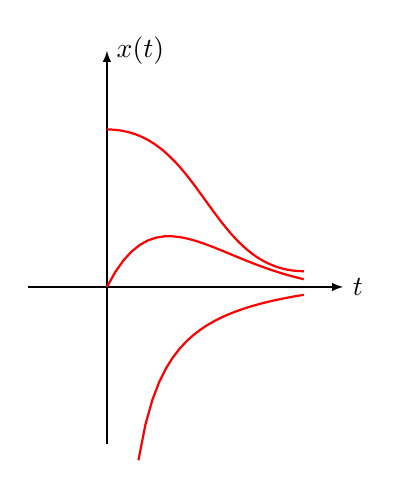
\begin{tikzpicture}[>=latex]
	\draw [->] (-1,0) -- (3,0) node [right] {\(t\)};
	\draw [->] (0,-2) -- (0,3) node [right] {\(x(t)\)};
	\draw [thick , red] (0,2) to [out=0 , in=180] (2.5,0.2);
	\draw [thick , red , domain=0:2.5] plot(\x , {2*sin(\x r) * exp(-\x)});
	\draw [thick , red , domain=0.4:2.5] plot(\x , {-1/\x+0.3});
\end{tikzpicture}

\end{document}
